% -------------------- Information --------------------

\newcommand{\TITLE}{Portable Document Format}
\newcommand{\AUTHOR}{Jason Chen}
\newcommand{\SUBJECT}{Public Speaking}
\newcommand{\KEYWORDS}{}
\newcommand{\INSTITUTE}{School of Mathematical Sciences, Tongji University}

% -------------------- Packages --------------------

\documentclass[xcolor=dvipsnames]{beamer}
\usepackage{amsmath}
% \usepackage{amsthm} % loaded by beamer.
\usepackage{amssymb}
\usepackage{commath} % abs, norm
\usepackage[mathscr]{euscript}
\usepackage{float} % 你们这帮float给我乖乖听话 HHHHHHHHHHH.
\usepackage{fontspec}
\usepackage{graphicx}
% \usepackage{hyperref} % loaded by beamer.
\usepackage{mathtools} % \xleftrightarrow.
\usepackage[timeinterval=1, font=Times, resetatpages=2]{tdclock}
\usepackage[absolute, overlay]{textpos}
\usepackage{tikz}
% \usepackage{xcolor} % loaded by beamer.
\usepackage[printwatermark]{xwatermark} % Foreground Watermarks.
\usepackage[all, cmtip]{xy}

% -------------------- Settings --------------------

% Package: beamer

\transpush<2>[duration=2]
\usetheme{Berlin}

% Package: graphicx

\graphicspath{{resources/}} % 图像文件目录

% Package: hyperref

\hypersetup{
    linktoc             =   all,
    colorlinks          =   true,
    linkcolor           =   cyan,
    anchorcolor         =   black,
    citecolor           =   green,
    filecolor           =   cyan,
    menucolor           =   red,
    runcolor            =   filecolor,
    urlcolor            =   magenta,
    pdftitle           	=   {\TITLE},
    pdfauthor          	=   {\AUTHOR},
    pdfsubject         	=   {\SUBJECT},
    pdfcreator			=	{Visual Studio Code},
    pdfproducer			=	{XeLaTeX with documentclass beamer},
    pdfkeywords        	=   {\KEYWORDS},
    bookmarksnumbered   =   true,
    pdfstartview        =   Fit,
    pdfpagelayout       =   OneColumn,
    pdfpagemode			=   FullScreen
}

% Package: tdclock

\newcommand{\FrameTextCrono}[1]{
    \begin{textblock*}{\paperwidth}(\textwidth + 1em, \textheight + 1em)
        #1
    \end{textblock*}
}

\newcommand{\FrameTextResetCrono}[1]{
    \begin{textblock*}{\paperwidth}(\textwidth + 1.5em, \textheight - 0.5em)
        #1
    \end{textblock*}
}

\newcommand{\ResetCronoBox}{\resetcrono{\fbox{reset}}}

\let\oldframe\frame
\let\oldendframe\endframe
\renewenvironment{frame}
    {\oldframe\FrameTextCrono{\small\color{blue}{\crono}}}
    {\oldendframe}

\let\oldtitlepage\titlepage
\renewcommand{\titlepage}{\oldtitlepage\FrameTextResetCrono{\ResetCronoBox}}

% Package: xwatermark

\newsavebox\mybox
\savebox\mybox{\tikz[color=cyan, opacity=0.2]\node{\fontspec{Comic Sans MS}\SUBJECT};}
\newwatermark*[
    allpages,
    angle=45,
    scale=3,
    xpos=0,
    ypos=0
]{\usebox\mybox}

% Title

\title{\TITLE}
\author{\AUTHOR}
\date{\tdyear\dateseparator\tdmonth\dateseparator\tdday\hspace{1em}\tdtime}
\institute{\INSTITUTE}
\titlegraphic{
\includegraphics[width=0.1\paperwidth]{tongji.jpg}}

% Theorem Environments

\let\note\undefined
\newtheorem{note}{Note}[section]

% -------------------- General new commands --------------------

\DeclareMathAlphabet{\mathsfsl}{OT1}{cmss}{m}{sl}

% Expectation

\newcommand{\expect}{\operatorname{E}\expectarg}
\DeclarePairedDelimiterX{\expectarg}[1]{(}{)}{
  \ifnum\currentgrouptype=16 \else\begingroup\fi
  \activatebar#1
  \ifnum\currentgrouptype=16 \else\endgroup\fi
}

\newcommand{\innermid}{\nonscript\;\delimsize\vert\nonscript\;}
\newcommand{\activatebar}{
  \begingroup\lccode`\~=`\|
  \lowercase{\endgroup\let~}\innermid
  \mathcode`|=\string"8000
}

\newcommand{\diff}{\mathop{}\!\mathrm{d}}
\newcommand{\matr}[1]{\ensuremath{\mathsfsl{#1}}} % italic sans serif
\newcommand{\me}{\mathrm{e}}
\newcommand{\mi}{\mathrm{i}}
\newcommand{\restrict[1]}{\raisebox{-.5ex}{$|$}_{#1}}
\newcommand{\vect}[1]{\bm{#1}}

% -------------------- Specific new commands --------------------



% -------------------- Document --------------------

\begin{document}

    % -------------------- Title Page --------------------

    \begin{frame}
        \initclock
        \titlepage
        \pagenumbering{arabic}
    \end{frame}

    % -------------------- Contents --------------------

    \begin{frame}
        \frametitle{Contents}
        \tableofcontents
    \end{frame}

    % -------------------- Body --------------------

    \section{Introduction}

    \begin{frame}
        \frametitle{Background}
        \begin{itemize}
            \item PDF format was developed by Adobe in 1990s
                to present documents, including texts and images.
            \item Since then its features have been widely extended.
        \end{itemize}
    \end{frame}

    \section{Presenting Documents}

    \begin{frame}
        \frametitle{Presenting Documents}
        \begin{itemize}
            \item PDF format is widely used for saving and exchanging documents.
            \item Many books, essays, articles and slides are saved
                in PDF format.
            \item PDF format features in presenting documents
                in a manner independent of environment.
        \end{itemize}
    \end{frame}

    \begin{frame}
        \frametitle{Preserving Typesetting}
        PDF files keep typesetting of documents.
        \begin{itemize}
            \item Texts, images and tables in PDF files will keep their positions
                so that the document looks the same
                whenever the application software, hardware,
                and operating systems are changed.
            \item While PPT format does not have such a feature.
                One may try his best to fit the title into one line
                in personal laptap, only to find out the title ranging in two
                lines when presenting the ppt to his audience. That is really
                frustrating.
        \end{itemize}
    \end{frame}

    \begin{frame}
        \frametitle{Preserving Typesetting (Continued)}
        % TODO: Add an example picture.
    \end{frame}

    \begin{frame}
        \frametitle{Containing All Needed Files}
        PDF files contains all files needed to present the documents.
        \begin{itemize}
            \item For example, font files are embedded in PDF files so that
            texts will present well even if the specific font isn't installed
            in the displaying device.
            \item {\fontspec{Berlin Sans FB Demi}Berlin Sans FB Demi,}
            {\fontspec{Bradley Hand ITC}Bradley Hand ITC,}
            {\fontspec{Colonna MT}Colonna MT,}
            {\fontspec{Curlz MT}Curlz MT,}
            {\fontspec{Edwardian Script ITC}Edwardian Script ITC,}
            {\fontspec{Euclid Fraktur}Euclid Fraktur,}
            {\fontspec{Forte}Forte,}
            {\fontspec{Freestyle Script}Freestyle Script,}
            {\fontspec{Harlow Solid Italic}Harlow Solid Italic,}
            {\fontspec{Mistral}Mistral,}
            {\fontspec{Snap ITC}Snap ITC.}
        \end{itemize}
    \end{frame}

    \begin{frame}
        \frametitle{Containing All Needed Files (Continued)}
        I took the screenshot when I was opening our lecture ppt on my iPad
        using Keynote.
        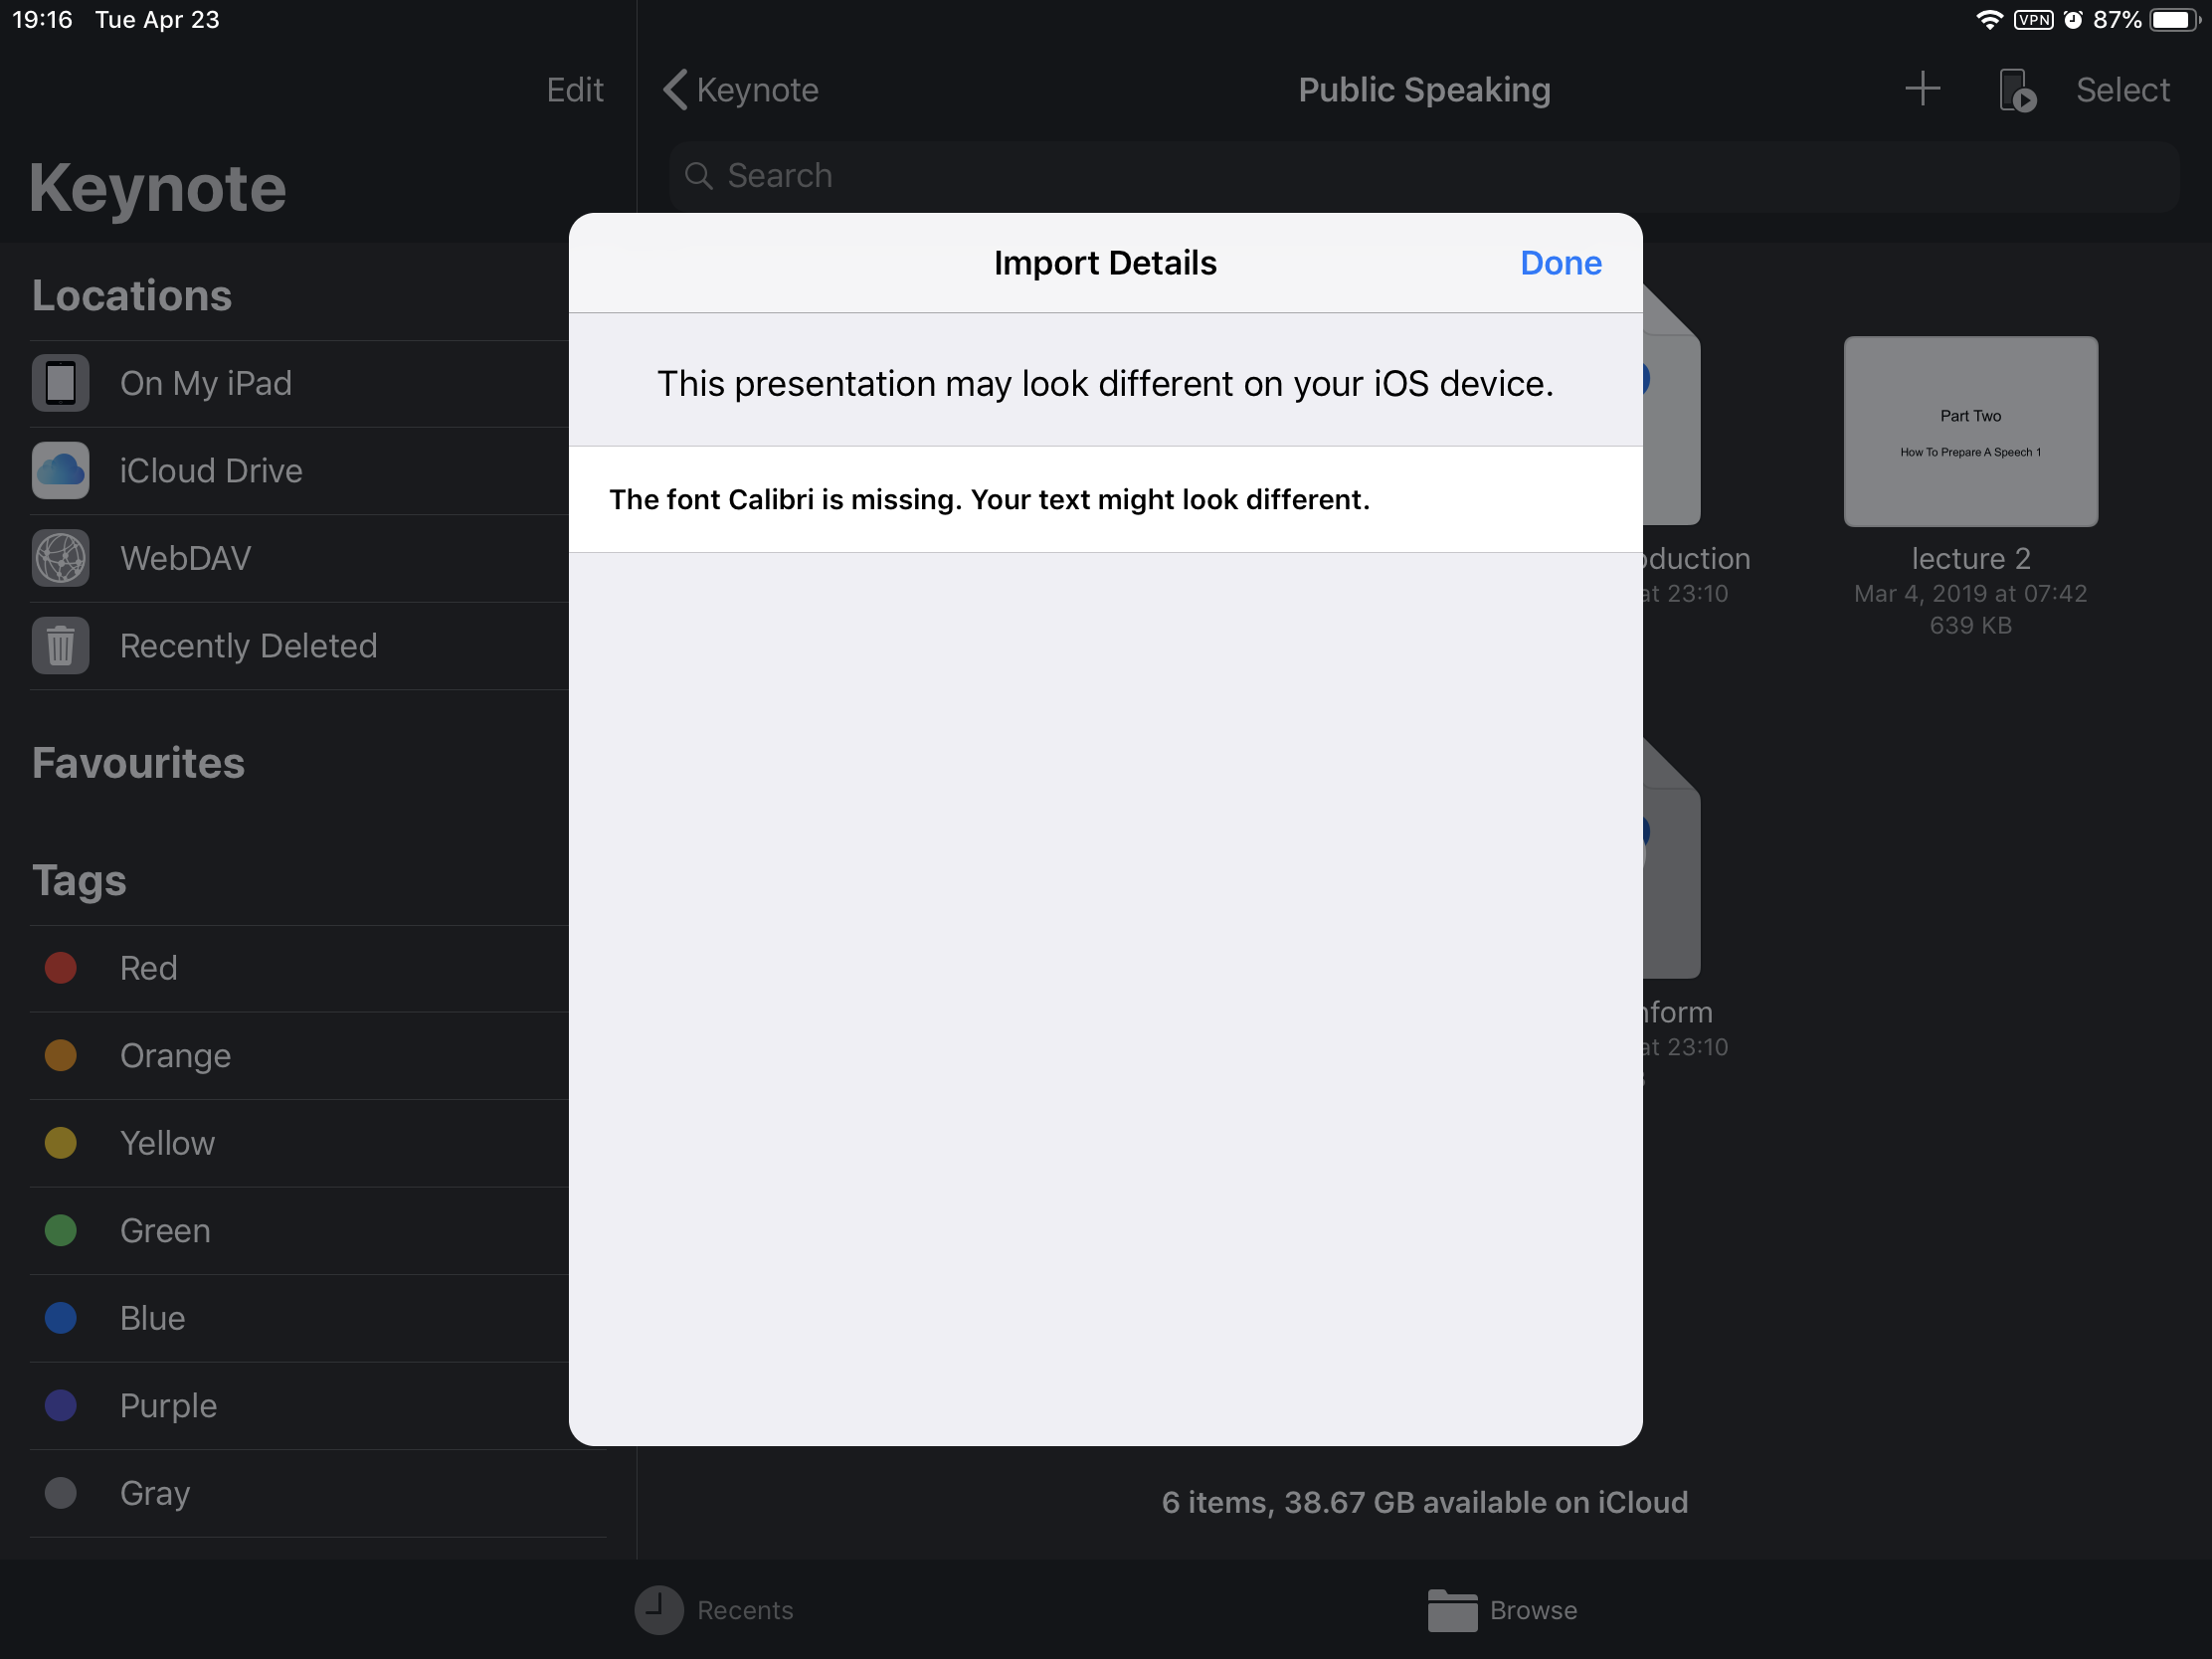
\includegraphics[scale=0.09]{missing_fonts.png}
    \end{frame}

    % TODO: new features including forms, rich media and so on.

    \section*{}

    \begin{frame}
        \FrameTextResetCrono{\ResetCronoBox}
        \centering\Huge{\fontspec{Palace Script MT}Thank You For Listening!}
    \end{frame}
\end{document}